% !TeX root = ../main.tex
% Add the above to each chapter to make compiling the PDF easier in some editors.

\chapter{Results}\label{chapter:results}
In this chapter, the results of the in \autoref{sec:analysis-tools} computed experinments are
presented. As previously described, three different video and image detection tools were used
to detect deepfakes. Calculations for the video detection tools were based on the
FaceForensics++ dataset, along with deepfake videos produced by DeepFaceLab and FaceSwap.
Image detection tools were evaluated using images created by FaceApp and Stable Diffusion,
as well as 20 authentic images.

\section{Comparative Results of tools}

\begin{figure}[htbp]
	\centering
	\begin{subfigure}{0.48\textwidth}
		\centering
		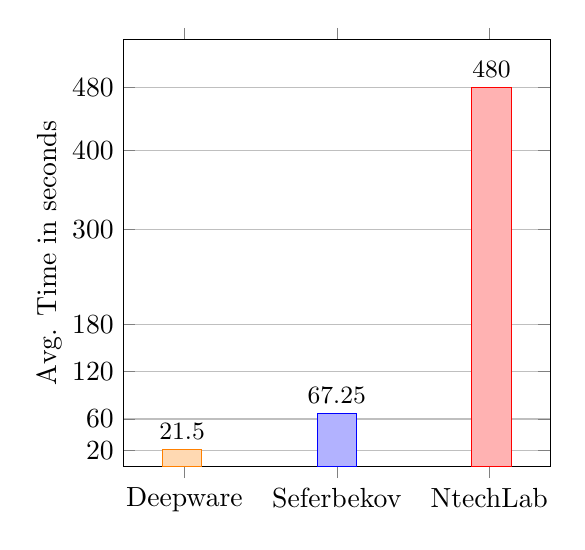
\begin{tikzpicture}
			\begin{axis}[
					ybar,
					bar width=5mm,
					width=7cm,
					height=7cm,
					enlarge x limits=0.2,
					legend style={at={(0.5,-0.2)},
							anchor=north,legend columns=-1},
					ylabel={Avg. Time in seconds},
					ylabel shift=-3pt,
					symbolic x coords={Deepware, Seferbekov, NtechLab},
					xtick={Deepware, Seferbekov, NtechLab},
					ytick={20,60,120,180,300,400,480},
					ymin=0,
					ymax=540,
					ymajorgrids=true,
					nodes near coords,
					every node near coord/.append style={font = {\fontsize{9 pt}{12 pt}\selectfont},color=black},
				]
				\addplot [orange,fill=orange!30,bar shift=-0.3mm] coordinates {(Deepware,21.5)};
				\addplot [blue,fill=blue!30] coordinates {(Seferbekov,67.25)};
				\addplot [red,fill=red!30, bar shift=0.3mm] coordinates {(NtechLab,480)};
			\end{axis}
		\end{tikzpicture}
		\caption{Video detection}
	\end{subfigure}
	\hfill
	\begin{subfigure}{0.48\textwidth}
		\centering
		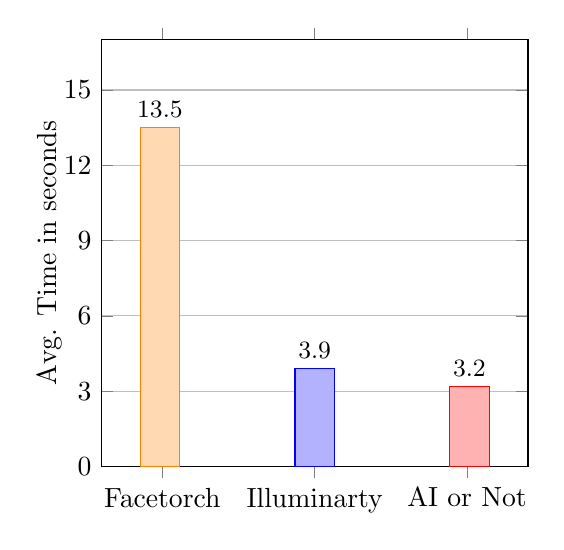
\begin{tikzpicture}
			\begin{axis}[
					ybar,
					bar width=5mm,
					width=7cm,
					height=7cm,
					enlarge x limits=0.2,
					legend style={at={(0.5,-0.2)},
							anchor=north,legend columns=-1},
					ylabel={Avg. Time in seconds},
					ylabel shift=-6pt,
					symbolic x coords={Facetorch, Illuminarty, AI or Not},
					xtick={Facetorch, Illuminarty, AI or Not},
					ytick={0,3,6,9,12,15},
					ymin=0,
					ymax=17,
					ymajorgrids=true,
					nodes near coords,
					every node near coord/.append style={font = {\fontsize{9 pt}{12 pt}\selectfont},color=black},
				]
				\addplot [orange,fill=orange!30,bar shift=-0.3mm] coordinates {(Facetorch,13.5)};
				\addplot [blue,fill=blue!30] coordinates {(Illuminarty,3.9)};
				\addplot [red,fill=red!30, bar shift=0.3mm] coordinates {(AI or Not,3.2)};
			\end{axis}
		\end{tikzpicture}
		\caption{Image detection}
	\end{subfigure}
    \caption{Comparison of the Processing Time of detection tools from~\autoref{sec:analysis-tools}}\label{fig:processing-time}
\end{figure}

From~\autoref{fig:processing-time}, it's evident that image detection tools process data faster
than the video detection tools. This discrepancy is due to the nature of the tools:
image detection tools only process a single image (frame), whereas video detection tools may 
need to break a video into numerous frames and analyze each one separately, which is considerably
more time-consuming. Additionally, among the video detection tools, NtechLab's tool was slower than 
both Deepware and Seferbekov's tool. This might be because of the detection techniques they used.

The duration a tool takes to process data is tied to the size of the input. For instance, 
Seferbekov's tool, when handling a video under 10MB, averaged a processing time of 20 seconds. However,
when confronted with a video exceeding 70MB, the time nearly tripled to almost a minute. 
The size-to-time relationship is consistent across all tools, meaning the larger the size of the
input, the longer it's going to take the tool to process it.

A comparison of assessed metrics for video detection tools is displayed in~\autoref{fig:comparison_video}.
The comparison of which tool performed better is interesting. As we know, accuracy and precision 
are defined as follows: Accuracy measures the fraction of all instances that are correctly 
identified and precision measures the fraction of instances that were correctly predicted as 
positive out of all predicted positives. So precision is especially important when the number
of false positives is high. In both of these cases NtechLab performed than the other two 
tools. This is due to the fact that NtechLab could detect more deepfakes.

Recall, also known as sensitivity, measures the proportion of actual positives that were 
correctly identified. It is crucial when the cost of missing a pisitive instance is high.
And F-1 Score is a metric providing a balance between preicision and recall, offering a more 
comprehensive view of the performance. While NtechLab had higher accuracy and precision, 
Deepware and Seferbekov's tool have caught up in terms of Recall and F1-Score. This suggests that
Deepware and Seferbekov's tool were more effective at correctly identifying true positive cases.

When it comes to image detection tools in~\autoref{fig:comparison_image}, AI or Not and 
Illuminarty outperformed Facetorch. One possible reason could be that AI or Not and 
Illuminarty are supported by companies and communities, receiving consisten updates. 
On the other hand, Facetorch is an open-source project. It hasn't had any updates 
since March 2023, which might make it less equipped to handle newer deepfake generation
techniques.

\begin{figure}[htbp]
	\centering
	\begin{subfigure}{0.48\textwidth}
		\centering
		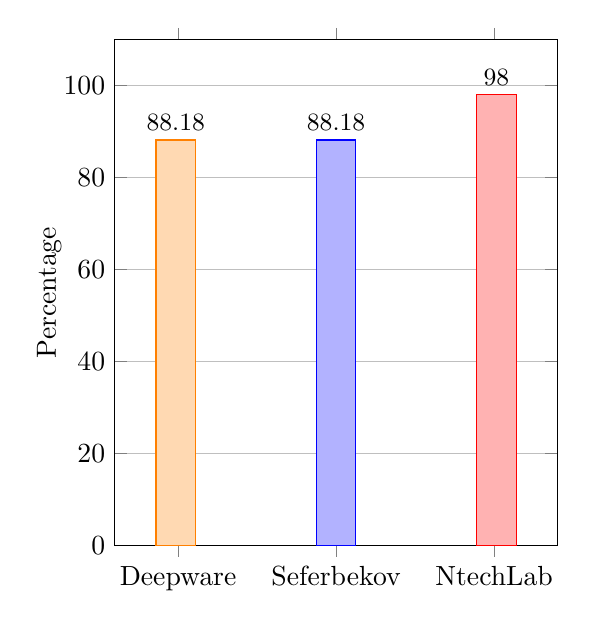
\begin{tikzpicture}
			\begin{axis}[
					ybar,
					bar width=5mm,
					width=7.2cm,
					height=8cm,
					enlarge x limits=0.2,
					legend style={at={(0.5,-0.2)},
							anchor=north,legend columns=-1},
					ylabel={Percentage},
					ylabel shift=-6pt,
					symbolic x coords={Deepware, Seferbekov, NtechLab},
					xtick={Deepware, Seferbekov, NtechLab},
					ytick={0,20,40,60,80,100},
					ymin=0,
					ymax=110,
					ymajorgrids=true,
					nodes near coords,
					every node near coord/.append style={font = {\fontsize{9 pt}{12 pt}\selectfont},color=black},
				]
				\addplot [orange,fill=orange!30,bar shift=-0.3mm] coordinates {(Deepware,88.18)};
				\addplot [blue,fill=blue!30] coordinates {(Seferbekov,88.18)};
				\addplot [red,fill=red!30, bar shift=0.3mm] coordinates {(NtechLab,98)};
			\end{axis}
		\end{tikzpicture}
		\caption{Detection accuracy}
	\end{subfigure}
	\hfill
	\begin{subfigure}{0.48\textwidth}
		\centering
		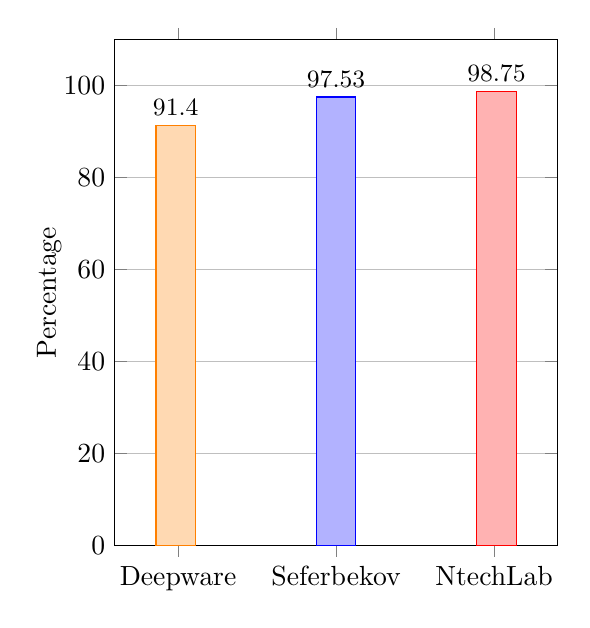
\begin{tikzpicture}
			\begin{axis}[
					ybar,
					bar width=5mm,
					width=7.2cm,
					height=8cm,
					enlarge x limits=0.2,
					legend style={at={(0.5,-0.2)},
							anchor=north,legend columns=-1},
					ylabel={Percentage},
					ylabel shift=-6pt,
					symbolic x coords={Deepware, Seferbekov, NtechLab},
					xtick={Deepware, Seferbekov, NtechLab},
					ytick={0,20,40,60,80,100},
					ymin=0,
					ymax=110,
					ymajorgrids=true,
					nodes near coords,
					every node near coord/.append style={font = {\fontsize{9 pt}{12 pt}\selectfont},color=black},
				]
				\addplot [orange,fill=orange!30,bar shift=-0.3mm] coordinates {(Deepware,91.40)};
				\addplot [blue,fill=blue!30] coordinates {(Seferbekov,97.53)};
				\addplot [red,fill=red!30, bar shift=0.3mm] coordinates {(NtechLab,98.75)};
			\end{axis}
		\end{tikzpicture}
		\caption{Precision}
	\end{subfigure}

    \vspace{0.5cm}

    \begin{subfigure}{0.48\textwidth}
		\centering
		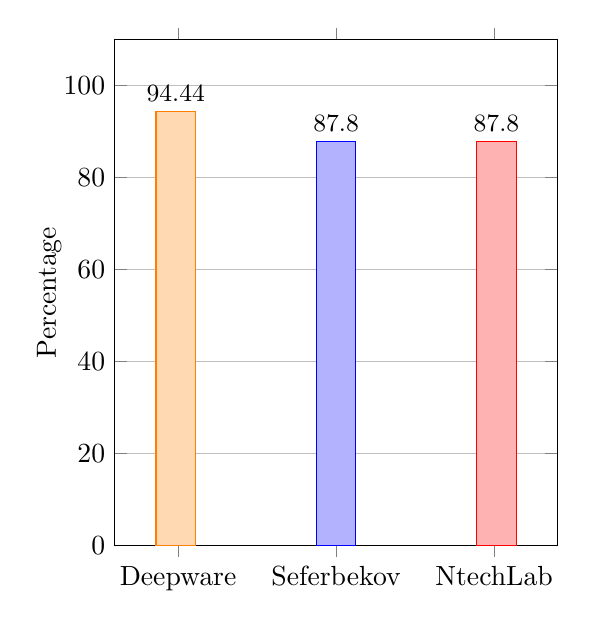
\begin{tikzpicture}
			\begin{axis}[
					ybar,
					bar width=5mm,
					width=7.2cm,
					height=8cm,
					enlarge x limits=0.2,
					legend style={at={(0.5,-0.2)},
							anchor=north,legend columns=-1},
					ylabel={Percentage},
					ylabel shift=-6pt,
					symbolic x coords={Deepware, Seferbekov, NtechLab},
					xtick={Deepware, Seferbekov, NtechLab},
					ytick={0,20,40,60,80,100},
					ymin=0,
					ymax=110,
					ymajorgrids=true,
					nodes near coords,
					every node near coord/.append style={font = {\fontsize{9 pt}{12 pt}\selectfont},color=black},
				]
				\addplot [orange,fill=orange!30,bar shift=-0.3mm] coordinates {(Deepware,94.44)};
				\addplot [blue,fill=blue!30] coordinates {(Seferbekov,87.8)};
				\addplot [red,fill=red!30, bar shift=0.3mm] coordinates {(NtechLab,87.8)};
			\end{axis}
		\end{tikzpicture}
		\caption{Recall}
	\end{subfigure}
	\hfill
	\begin{subfigure}{0.48\textwidth}
		\centering
		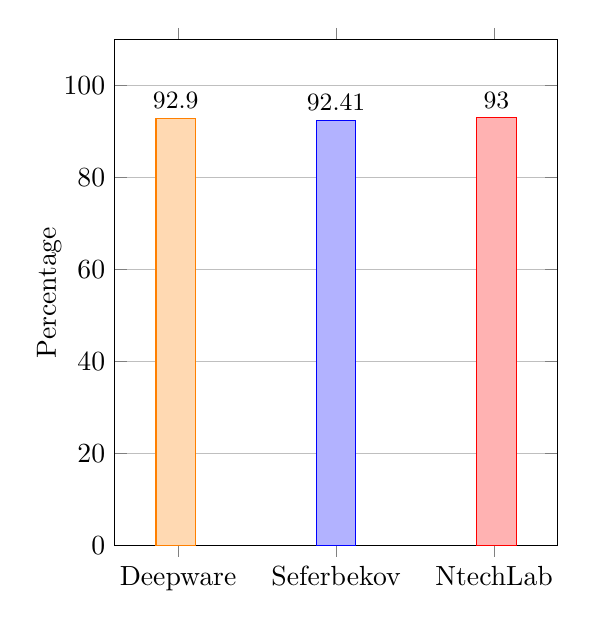
\begin{tikzpicture}
			\begin{axis}[
					ybar,
					bar width=5mm,
					width=7.2cm,
					height=8cm,
					enlarge x limits=0.2,
					legend style={at={(0.5,-0.2)},
							anchor=north,legend columns=-1},
					ylabel={Percentage},
					ylabel shift=-6pt,
					symbolic x coords={Deepware, Seferbekov, NtechLab},
					xtick={Deepware, Seferbekov, NtechLab},
					ytick={0,20,40,60,80,100},
					ymin=0,
					ymax=110,
					ymajorgrids=true,
					nodes near coords,
					every node near coord/.append style={font = {\fontsize{9 pt}{12 pt}\selectfont},color=black},
				]
				\addplot [orange,fill=orange!30,bar shift=-0.3mm] coordinates {(Deepware,92.9)};
				\addplot [blue,fill=blue!30] coordinates {(Seferbekov,92.41)};
				\addplot [red,fill=red!30, bar shift=0.3mm] coordinates {(NtechLab,93)};
			\end{axis}
		\end{tikzpicture}
		\caption{F1-Score}
	\end{subfigure}
    \caption{Comparison of video detection tools from~\autoref{sec:analysis-tools} according
    to the evaluation metrics listed in~\autoref{tab:evaluation_metrics}}\label{fig:comparison_video}
\end{figure}


\begin{figure}[htbp]
	\centering
	\begin{subfigure}{0.48\textwidth}
		\centering
		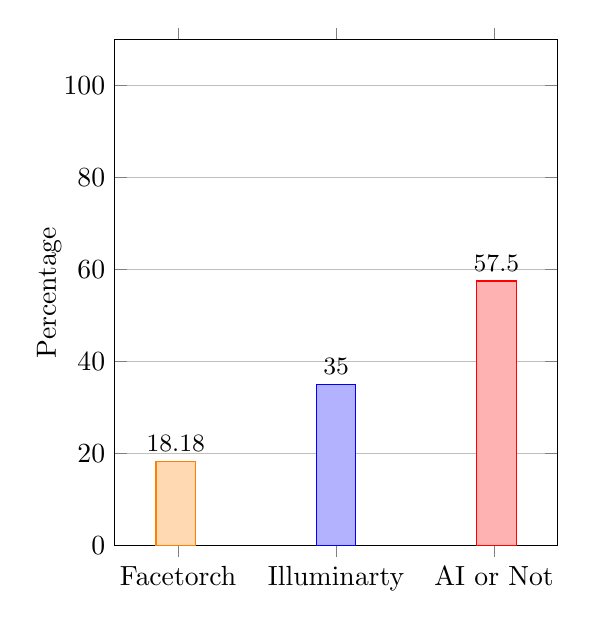
\begin{tikzpicture}
			\begin{axis}[
					ybar,
					bar width=5mm,
					width=7.2cm,
					height=8cm,
					enlarge x limits=0.2,
					legend style={at={(0.5,-0.2)},
							anchor=north,legend columns=-1},
					ylabel={Percentage},
					ylabel shift=-6pt,
					symbolic x coords={Facetorch, Illuminarty, AI or Not},
					xtick={Facetorch, Illuminarty, AI or Not},
					ytick={0,20,40,60,80,100},
					ymin=0,
					ymax=110,
					ymajorgrids=true,
					nodes near coords,
					every node near coord/.append style={font = {\fontsize{9 pt}{12 pt}\selectfont},color=black},
				]
				\addplot [orange,fill=orange!30,bar shift=-0.3mm] coordinates {(Facetorch,18.18)};
				\addplot [blue,fill=blue!30] coordinates {(Illuminarty,35)};
				\addplot [red,fill=red!30, bar shift=0.3mm] coordinates {(AI or Not,57.5)};
			\end{axis}
		\end{tikzpicture}
		\caption{Detection accuracy}
	\end{subfigure}
	\hfill
	\begin{subfigure}{0.48\textwidth}
		\centering
		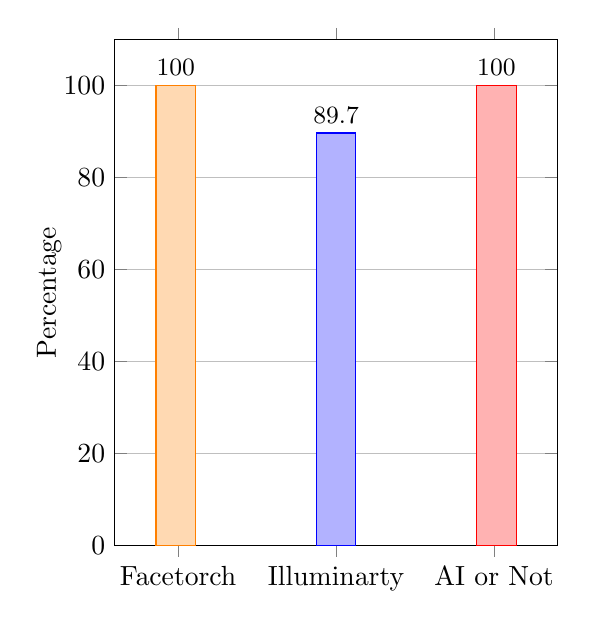
\begin{tikzpicture}
			\begin{axis}[
					ybar,
					bar width=5mm,
					width=7.2cm,
					height=8cm,
					enlarge x limits=0.2,
					legend style={at={(0.5,-0.2)},
							anchor=north,legend columns=-1},
					ylabel={Percentage},
					ylabel shift=-6pt,
					symbolic x coords={Facetorch, Illuminarty, AI or Not},
					xtick={Facetorch, Illuminarty, AI or Not},
					ytick={0,20,40,60,80,100},
					ymin=0,
					ymax=110,
					ymajorgrids=true,
					nodes near coords,
					every node near coord/.append style={font = {\fontsize{9 pt}{12 pt}\selectfont},color=black},
				]
				\addplot [orange,fill=orange!30,bar shift=-0.3mm] coordinates {(Facetorch,100)};
				\addplot [blue,fill=blue!30] coordinates {(Illuminarty,89.7)};
				\addplot [red,fill=red!30, bar shift=0.3mm] coordinates {(AI or Not,100)};
			\end{axis}
		\end{tikzpicture}
		\caption{Precision}
	\end{subfigure}

    \vspace{0.5cm}

    \begin{subfigure}{0.48\textwidth}
		\centering
		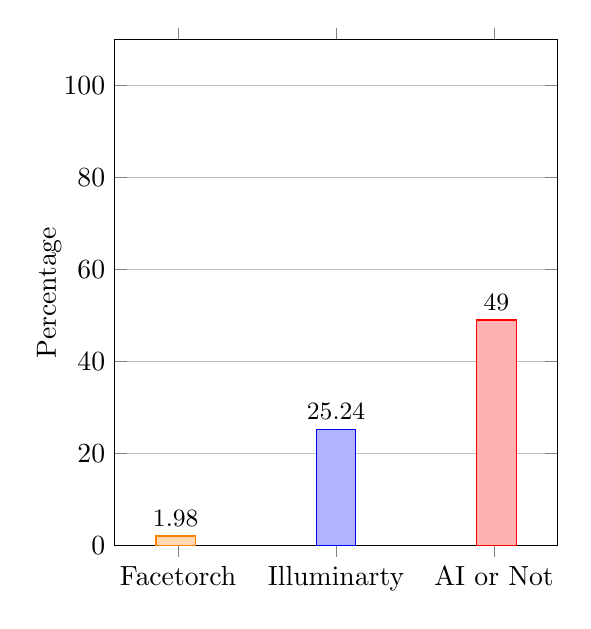
\begin{tikzpicture}
			\begin{axis}[
					ybar,
					bar width=5mm,
					width=7.2cm,
					height=8cm,
					enlarge x limits=0.2,
					legend style={at={(0.5,-0.2)},
							anchor=north,legend columns=-1},
					ylabel={Percentage},
					ylabel shift=-6pt,
					symbolic x coords={Facetorch, Illuminarty, AI or Not},
					xtick={Facetorch, Illuminarty, AI or Not},
					ytick={0,20,40,60,80,100},
					ymin=0,
					ymax=110,
					ymajorgrids=true,
					nodes near coords,
					every node near coord/.append style={font = {\fontsize{9 pt}{12 pt}\selectfont},color=black},
				]
				\addplot [orange,fill=orange!30,bar shift=-0.3mm] coordinates {(Facetorch,1.98)};
				\addplot [blue,fill=blue!30] coordinates {(Illuminarty,25.24)};
				\addplot [red,fill=red!30, bar shift=0.3mm] coordinates {(AI or Not,49)};
			\end{axis}
		\end{tikzpicture}
		\caption{Recall}
	\end{subfigure}
	\hfill
	\begin{subfigure}{0.48\textwidth}
		\centering
		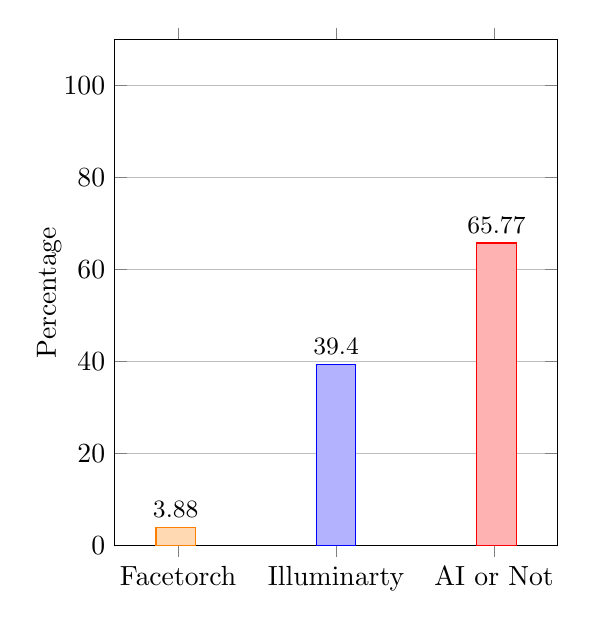
\begin{tikzpicture}
			\begin{axis}[
					ybar,
					bar width=5mm,
					width=7.2cm,
					height=8cm,
					enlarge x limits=0.2,
					legend style={at={(0.5,-0.2)},
							anchor=north,legend columns=-1},
					ylabel={Percentage},
					ylabel shift=-6pt,
					symbolic x coords={Facetorch, Illuminarty, AI or Not},
					xtick={Facetorch, Illuminarty, AI or Not},
					ytick={0,20,40,60,80,100},
					ymin=0,
					ymax=110,
					ymajorgrids=true,
					nodes near coords,
					every node near coord/.append style={font = {\fontsize{9 pt}{12 pt}\selectfont},color=black},
				]
				\addplot [orange,fill=orange!30,bar shift=-0.3mm] coordinates {(Facetorch,3.88)};
				\addplot [blue,fill=blue!30] coordinates {(Illuminarty,39.4)};
				\addplot [red,fill=red!30, bar shift=0.3mm] coordinates {(AI or Not,65.77)};
			\end{axis}
		\end{tikzpicture}
		\caption{F1-Score}
	\end{subfigure}
	\caption{Comparison of image detection tools from~\autoref{sec:analysis-tools} according
    to the evaluation metrics listed in~\autoref{tab:evaluation_metrics}}\label{fig:comparison_image}
\end{figure}


\section{Final Results}
To conclude the achieved results, it's noticable that some tools might have a high accuracy rate
but perform poorly in terms of recall and F1-Score. Contrarily, certain tools might demonstrate 
high precision but low recall, which might indicate that the tool misses some actual 
positives. By comparing these metrics across the testes tools, a clearer insight into their 
strengths and limitations can be gained. This, in turn, helps us make important decisions on
which tool is ideal for a particular task.
